\documentclass[margin=10pt]{standalone}
\usepackage{tikz}
\usepackage{pgfplots}
\usepackage{caption} % For captions


\usepackage{palatino}
\newlength{\mainwidth}
\setlength{\mainwidth}{460pt}

% Define the colors
\definecolor{color1}{HTML}{1b9e77}
\definecolor{color2}{HTML}{d95f02}
\definecolor{color3}{HTML}{7570b3}
\definecolor{color4}{HTML}{e7298a}
\definecolor{color5}{HTML}{66a61e}
\definecolor{color6}{HTML}{e6ab02}
\definecolor{color7}{HTML}{a6761d}



\begin{document}

\begin{minipage}[b]{0.48\mainwidth}
\centering
    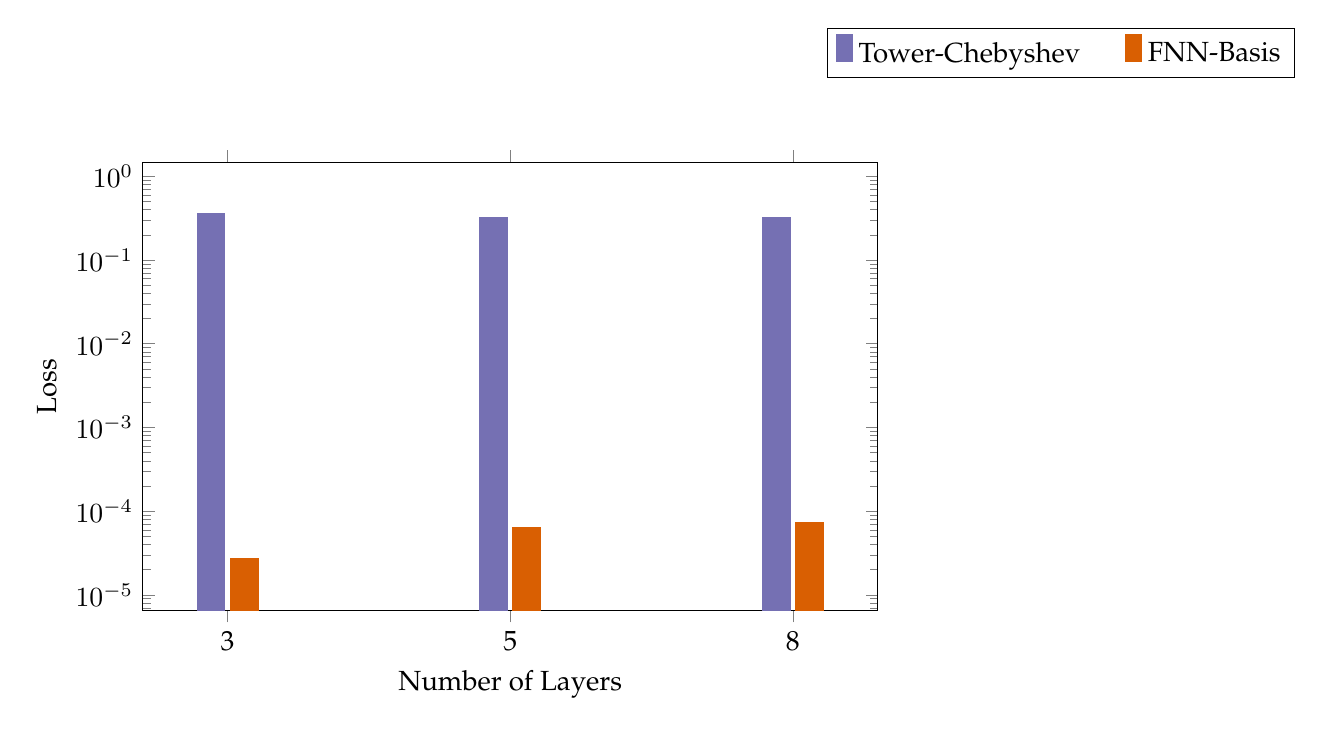
\begin{tikzpicture}
        \begin{axis}[
            ybar,
            bar width=10pt,
            enlargelimits=0.15,
            ylabel={Loss},
            xlabel={Number of Layers},
            symbolic x coords={3,5,8},
            xtick=data,
            ymode = log,
            log origin=infty,
            width=0.9 \textwidth,
            legend style={at={(1.25,1.3)},anchor=north,legend columns=2, /tikz/every even column/.append style={column sep=0.5cm}},
            legend image code/.code={
                        \draw [#1] (0cm,-0.1cm) rectangle (0.2cm,0.25cm); },
            height=0.6\textwidth,
        ]
        \addplot+[color=color3] coordinates {
            (3,0.3559075891971588)
            (5,0.3203471302986145) 
            (8,0.3203469216823578)
        };
        \addlegendentry{Tower-Chebyshev}

        \addplot+[color=color2] coordinates {
            (3,2.7030513592762873e-05) 
            (5,6.306666666666666e-05)
            (8,7.37241207389161e-05)
        };
        \addlegendentry{FNN-Basis}
        \end{axis}
    \end{tikzpicture}
\end{minipage}
\hfill
\begin{minipage}[b]{0.48\mainwidth}
    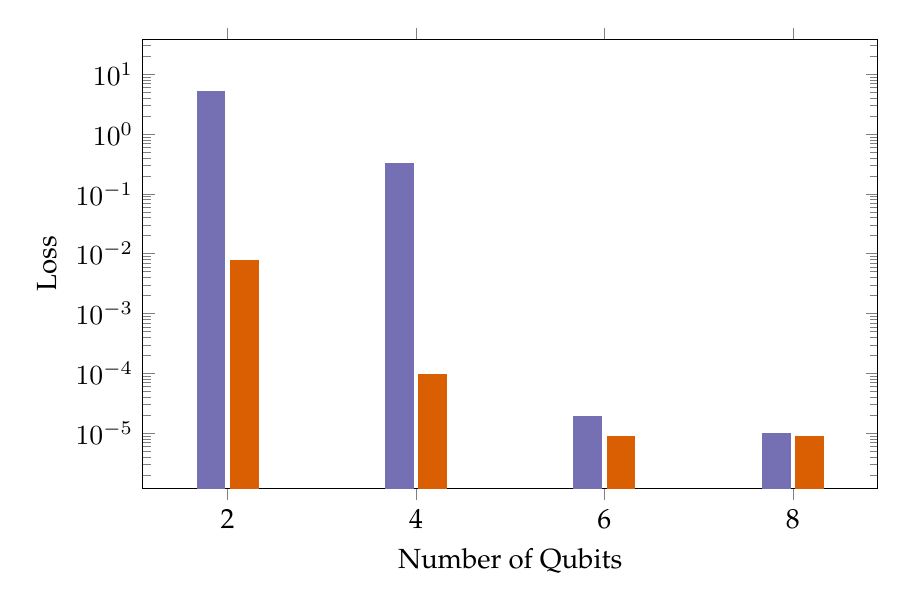
\begin{tikzpicture}
        \begin{axis}[
            ybar,
            bar width=10pt,
            enlargelimits=0.15,
            ylabel={Loss},
            xlabel={Number of Qubits},
            symbolic x coords={2, 4, 6, 8},
            xtick=data,
            ymode=log,
            log origin=infty,
            width=0.9\textwidth,
            max space between ticks=25,
            height=0.6\textwidth,
        ]
        \addplot+[color=color3] coordinates {(2,5.1607) (4,0.3203) (6,1.8885e-05) (8,9.6682e-06)};
        \addplot+[color=color2] coordinates {(2,0.0077) (4,9.7179e-05) (6,8.8285e-06) (8,8.8918e-06)};
    \end{axis}
\end{tikzpicture}
\end{minipage}


\end{document}
